% Chapter 1

\chapter{Introduction} % Write in your own chapter title
\label{Chapter1}
\lhead{Chapter 1. \emph{Introduction}} % Write in your own chapter title to set the page header

\section{Introduction}
\subsection{Overview of Project}
Outdoor and indoor localization is an integral component of  IoT (Internet of Things) in this era of mobile computing. Indoor localization can open new horizons for ubiquitous applications targeting university departments, government small institutes, software houses, airports, shopping malls, museums etc. Our project will find the location of a specific person by using appropriate machine learning approach using BLE based Android application. This location will be used to provide guided tour of the indoor building (Computer Science and Engineering Department at UET, Lahore) we will use to validate our work. 

This project will guide persons who are not much familiar with visiting place. It has an android application that will predict the indoor location of a person at room level and also gives information of current room location and nearby rooms in the form of text, images, audio and videos. In our case visiting place will be CSE dept at UET LHR. For room prediction, RSSI fingerprints of BLE beacons will be captured for training of model. After finding the location of the person, guidelines of that certain room/area will be provided to the user on user end Android application. Indoor positioning has numerous applications. We can use indoor positioning of people to guide them inside shopping malls, airports or museums. 


Indoor positioning systems can be broadly classified into two main parts: Systems that need some infrastructure which are further categorized into those which needs ad-hoc deployment  like BLE beacons and systems which takes profit of previously installed infrastructure like WiFi fingerprinting technique. Those technologies which do not need any infrastructure deployment are based on magnetic field fingerprinting. Ad-hoc deployment can be initiate in new areas where there is need to save environment from magnetic rays or in those areas where WAPs are weak so we choose to detect indoor location using BLE beacons.Also,  BLE based indoor  localization is wireless, consumes low power because it works on battery and mostly available in smart mobile devices.

BLE can be used from two different approaches: trilateration and fingerprinting. In tilateration relationship between the user's RSSI measurement and its distance to the BLE beacon station is considered. By estimating distances to multiple beacon stations, the user's location can be predicted using a least square algorithm. The  fingerprinting approach is implemented in two phases: an ofliine phase and an online phase. The ofline phase is called the training phase. During this phase, fingerprint  RSSI values are determined of every beacon from each device location. The online phase is known as the localization phase which is the actual prediction of the user's device location.

\textbf{What are BLE beacons?}

Beacons are small, wireless transmitters that use low-energy Bluetooth technology to send signals to other smart devices nearby.They are probably the most recent advancement in area innovation and closeness advertising. Set forth plainly, they associate and transmit data to savvy devices making area based prediction and are progressively precise.Each tool contains a CPU, radio, and batteries, and it really works by means of again and again broadcasting out an identifier. This identifier is picked up by way of your tool, commonly a cellular, and marks out an crucial area for your surroundings. The identifier is a unique ID variety that your phone recognizes as specific to the beacon. Once related, the beacon will carry out the signals for what we are using it. 
\begin{figure}[h]]
\begin{center}
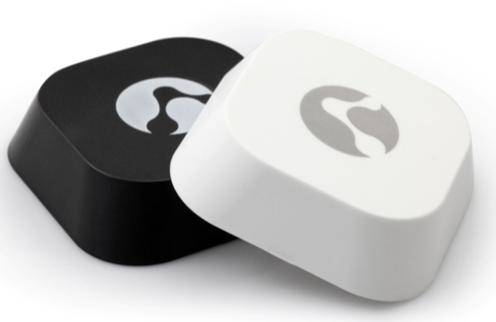
\includegraphics[scale=0.6]{beacon}
\caption{Beacons}
\label{fig:1}
\end{center}
\end{figure}


\textbf{Why we are using BLE beacons?}

In this evergoing techinal era, everyone wants leisure and his needs in less time and cost. He wants to become smart.So, due to mentioned reasons we are using this technology.
\begin{itemize}
\item Beacons are small, wireless sensors that are normally placed in a casing, have low power consumption because they work on battery.
\item The technology uses Bluetooth Low Energy (also called Bluetooth Smart or Bluetooth Version 4.0+) to broadcast radio signals or, simply put, to communicate with other smart devices.
\item The broadcasted beacon signals can be captured by smart gadgets, like phones, to call ad-hoc actions.
\item Under the beacon’s casing, there is a small ARM computer with a Bluetooth Smart connectivity module, which is powered by a battery.
\item The module runs on firmware, a piece of software installed on beacons.
\item As the computing power is limited, it can be used for processing sensor data (information about signal power) and encrypting a beacon’s ID. There is a small antenna from the CPU.
\item The antenna is built in to broadcast electromagnetic waves with specific length and frequency (2.4 GHz radio waves).
\item This technology is primarily used for mapping and location services using the RSSI (received signal strength indicator) estimate. 
\end{itemize}

\subsection{Background}
Outdoor localization has been formalized by using satellite-based technologies i.e. GPS\cite{GPS}, BeiDou\cite{cooper2016loco}, GLONASS\cite{cooper2016loco}, and GALILEO\cite{GALILEO}. It is hard for finding the indoor location by using conventional GPS technology because of no direct (Line of Sight)\cite{akram2018censloc} in indoors, so we cannot use these technologies for indoor positioning. Up to date, the technologies used for indoor localization approach are: TOA (Time of Arrival), TDOA (Time Difference of Arrival), AOA (angle of arrival) but they have some limitations. TOA and TDOA require precise clock count and its synchronization and AOA-based systems require special antennas for their propagation. 
By keeping in view the evergreen trend of engaging users towards something is through mobile computing.So, there exists some systems which used magnetic rays, time of arival of specific signals, some used WiFi based localization and also deployed on Apple and Android smart phones but due to coherence and interference of different signals in determining the RSSI of fixed WAPs, crucial errors occurred. By analyzing these calculations, we are able to avoid multiiteration(which predict location of device by determining the distance between the AP and mobile device) and capture fingerprints from multiple mobile devices.

The indoor positioning system which we are using is communicating with hardware device so we require a technique which translates the signal into a location. There are three categories to transform this: proximity, geometric and scene analysis,. Proximity methods create zones and assigns the users location when they enter that zone. Geometric method uses signal measurements from device locations and put them in geometrical equations to predict the location but scene analysis method measures the signal from different refence points by standing at one location and then predicts location by passing that fingerprint to trained model which is called fingerprinting technique. A fingerprint is
a collection of signals received at a certain location in the scene, in this way they aim to make the fingerprint
location specific, such fingerprints are often based on the RSSI values collected from beacons.

So, we are going to implement a system which employs suitable machine learning approach to find the location by using RSSI (Received Signal Strength Indicator) fingerprinting technique because there is less hinderance of other signals in using this technique.. This RSSI values will pass to the trained model (a model which is trained on a given set of input and output values by using appropriate machine learning algorithm) which gives the location of the user's mobile device.



\section{Motivation} 
People/visitors who go to an unknown place find it difficult to traverse and wants to find places/people of interest easily. Such problems motivate us to provide ease and leverage facility to users so that they can see the information of a particular indoor environment on his mobile application automatically. BLE is available on nearly every smart device so no additional hardware required at user end. Hence by utilizing their indoor location determined using machine learning on BLE fingerprints, guided tours of smart campus to visitors can be provided and facilitating them. We are using latest technology of BLE beacons because they work on battery and consume less energy than Wi-Fi signals\cite{hultgren2015evaluating}.

\section{Objectives of the project}
\subsection{Industry Objectives}
\begin{itemize}
\item Implement a system that takes into account the demands of university campus exploration.
\item This project leads to visitors of any organization or store to save their time and effort by providing them textual and pictorial information of organization or store.
\item Administrators seek advantage of their time by providing much information to their customers in less time which automatically increase the sales and profit of their product.

\end{itemize}
\subsection{Research Objectives}
\begin{itemize}
\item To find the location of the user that will be connected to his Android app via Bluetooth technology\cite{Introduction}.
\item To monitor and provide guidelines to user who is connected to the BLE beacon via Bluetooth and mobile application, we need to find user location inside buildings.
\item To understand the concept of Android application development which provide textual and pictorial information of particular area and its nearby areas to the user who is located in that indoor environment.


\end{itemize}
\subsection{Academic Objectives}
\begin{itemize}
\item This project enables us to understand the concepts of following subjects:
\\a.	Machine learning
\\b.	Networking
\\c.	Android development
\\d.	Front-end design
\\e.	Client server communication management
\item To complete a whole real world project , utilizing concepts from computer networking, databases, machine learning, software development life cycle of SE , testing and mobile development.
\item To develop the understanding and connection between the Android app and the hardware structure. 
\item To find the best Machine Learning algorithms which are used to train the model of fingerprints. 
\item To make an Android application which use as an interface to provide guidelines to the user who is located in a particular indoor environment.
\item To ensure the use of latest technologies in implementing the project which helps technical persons and students to enhance their academic skills via learning new features


\end{itemize}

\section{Scope of the project}
In this project, android application runs on a user’s mobile device and and will capture BLE RSSI fingerprints. The fingerprints collected at the initial stage will be processed and used to train suitable machine learning model, after training of the ML based location prediction model, based on the room prediction relevant information of nearby rooms, facilities and personnel available will be prepared to be displayed to user at run time , the user will be guided to install our Android app on their phone, their mobile device will capture BLE fingerprint and the fingerprint will be sent to back end server where our trained model will predict their current location inside building in terms of room\cite{Loco}. The relevant information will be delivered and shown on user mobile device providing guided tour. 
The placement of Bluetooth low energy beacons will be held in CSE dept at UET Lahore. 


\section{Target Audience}
Targeted audience will be the:
\begin{itemize}
\item Visitors of the University campus 
\item New Students and Staff of the campus
\end{itemize}



\section{Possible Applications of work}
The possible application of work for our project are as follows:


\begin{itemize}
\item Software house information (Development, QA, Frontier)
\item Airport assisting system
\item University Campus smart information system
\item Government small Institutes
\item Medical departments exploration in hospitals
\end{itemize}


\begin{table}[h]
\centering
\begin{tabular}{l|l} \hline
\end{tabular}
%\caption{Flow in the logic}
\label{tab:logic_flow}
\end{table}




